\documentclass[acmtog]{acmart}
\usepackage{graphicx}
\usepackage{subfigure}
\usepackage{natbib}

% Title portion
\title{Assignment 5 : Volume Rendering} 
\author{Chenghua Yang \quad 2019533089 \quad yangchh@shanghaitech.edu.cn}

% Document starts
\begin{document}
\maketitle

\vspace*{2 ex}


\section{Introduction}

In this assignment, I realise a navie volume renderer using analysis geometry.

\section{Implementation Details}

\subsection{The value and gradient}
Given a position in a specified geometry equation field, the isovalue and gradient of this point can be easily obtained by the iso function and its derivative function.\\ 
I used matlab to get the gradient(The 3 partial deriviations) and straightly translate it into C++ code.\\
\begin{figure}[h]
        \centering
        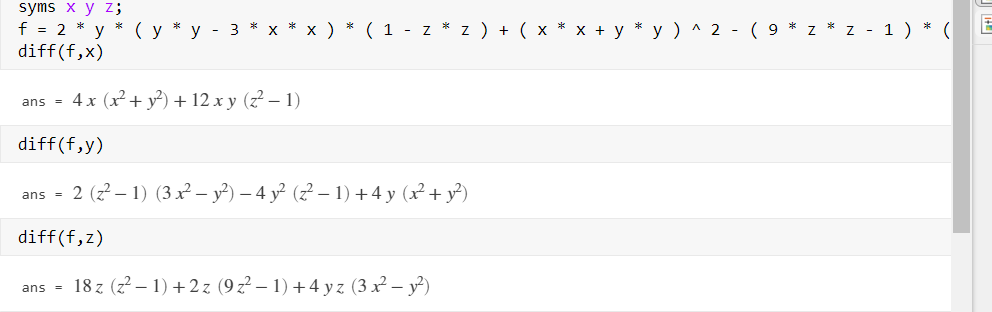
\includegraphics[width=10cm,height=4cm]{matlab.png}
        \caption{The matlab syms function diff function}
\end{figure}

\subsection{The transfer function}
Given a position, a isovalue and its gradient, th transfer function is able to give a color for this point for rendering.
The color of the point need to be defined manually. Here in the result, I use the length of gradient to determine the color and add the phong lighting model to make it more visible.\\
It's ok to use delta function or guassian function to get the alpha value of this position (i.e. the closer the isovalue to the render value , the more opacity the point will be). However, considering that in this assignment we only want to render is just one isovalue, I use a step combiend function to handle this. I will explain it later.\\

\begin{figure}[h]
        \centering
        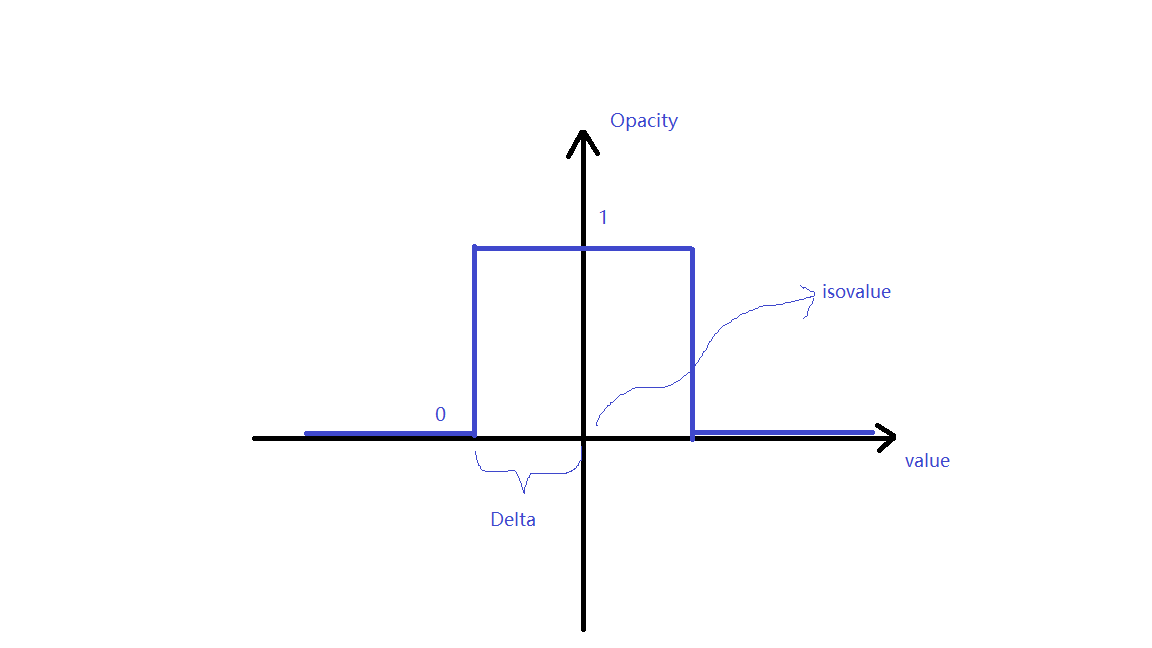
\includegraphics[width=7cm,height=3cm]{Step.png}
        \caption{The step functions used to determine rendering and opacity}
\end{figure}

\subsection{The renderer}
The normal render for a volume render need to sample a point in every step and accumulate colors through the way.\\
However, if we consider the geometry to be opacity at all, we actually only need the first point we encounter on the isosurface, when we get this point(i.e. some point whose value is close enough to the rendering value), we directly analysis it using transfer function and quit to get the color of this pixel. Therefore, the step function is used. 

\begin{figure}[h]
        \centering
        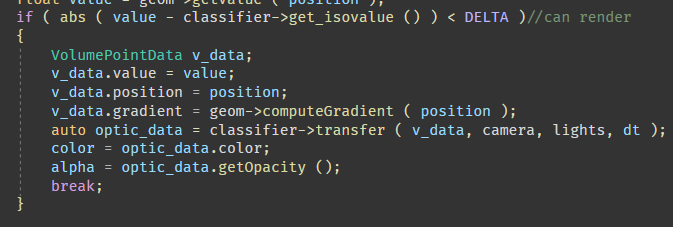
\includegraphics[width=6.5cm,height=2cm]{delta.png}
        \caption{The rendering process using step function with delta}
\end{figure}


\section{Results}

The accept delta have the main effect on the geometry shape. The three image use different delta to get a relatively nice result.

\begin{figure}[h]
        \centering
        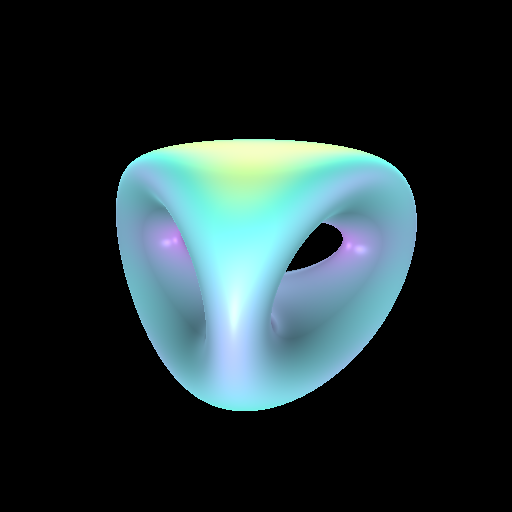
\includegraphics[width=8cm,height=8cm]{genus2.png}
        \caption{Genus2: using 0.1*gradient norm as color and 0.001f as delta}
\end{figure}

\begin{figure}[h]
        \centering
        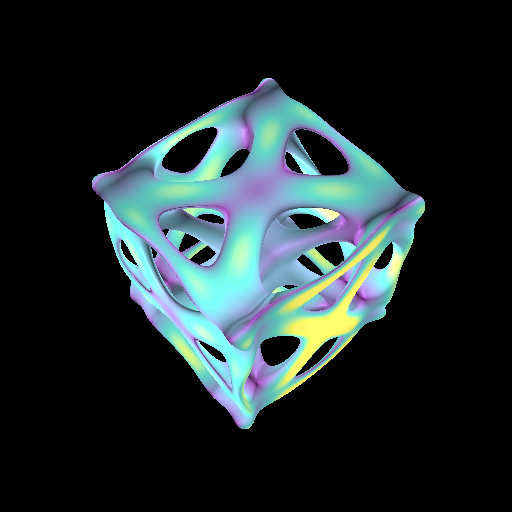
\includegraphics[width=8cm,height=8cm]{porous_surf.png}
        \caption{PorousSurf: using 0.5*gradient norm as color and 0.005f as delta}
\end{figure}

\begin{figure}[h]
        \centering
        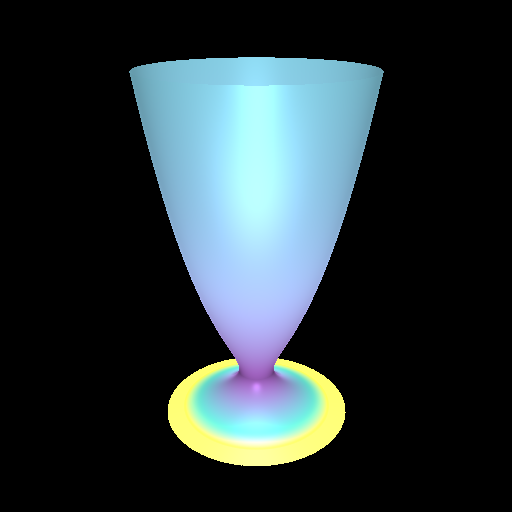
\includegraphics[width=8cm,height=8cm]{wineglass.png}
        \caption{WineGlass: using 0.5*gradient norm as color and 0.001f as delta}
\end{figure}

\section{Conclusion}

In this assignment, I learn about the transfer function and basic volume render process.

\end{document}
